\section{Adding New Services: Step-By-Step}
\begin{enumerate}
\item Make copies of the service template source and header files:
\begin{docspec}
    uxas/code/src/Services/00\_ServiceTemplate.cpp
\end{docspec}
\begin{docspec}
    uxas/code/src/Services/00\_ServiceTemplate.h
\end{docspec}
\item Change the name of the copied files to reflect the name of the new service.
\item In the new files, search for the string \textit{c00\_ServiceTemplate} and Replace it with the new service name.
\item Change the unique include guard entries in the header file, i.e. \textit{UXAS\_00\_SERVICE\_TEMPLATE\_H}, to match the new service name.
\item Edit the file:
\begin{docspec}
    uxas/code/src/Services/00\_ServiceList.h
\end{docspec}
to add entries for the new service:
\begin{enumerate}
  \item include the header file for the new service in the section labeled \textit{SERVICE HEADER FILES SECTION}, e.g.:
\begin{docspec}
\#include "CmasiAreaSearchTaskService.h"
\end{docspec}
  
  \item add a service registration string in the section labeled \textit{SERVICE REGISTRATION SECTION} e.g.:
\begin{docspec}
{auto svc = uxas::stduxas::make\_unique<afrl::cmasi::AreaSearchTask>();}
\end{docspec}
  \item if the new service is a task, include the header file of the corresponding task message in the section labeled \textit{INCLUDE TASK MESSAGES SECTION}, e.g.:
\begin{docspec}
\#include "afrl/cmasi/AreaSearchTask.h"
\end{docspec} 
  \item if the new service is a task, add a subscription string in the section labeled \textit{SUBSCRIBE TO TASKS SECTION}, e.g.:
\begin{docspec}
addSubscriptionAddress(afrl::cmasi::AreaSearchTask::AREASEARCHTASK\_FULL\_LMCP\_TYPE\_NAME);
\end{docspec} 
  \end{enumerate}  
\end{enumerate}


\section{Configuring Services}
Service are configured using a global configuration file written in XML. The configuration file is selected either  by using the default configuration file name: \textbf{\textit{cfg.xml}} or passing in the path/filename when starting UxAS:
\begin{docspec}
	uxas\_main \textbf{-cfgPath} \textit{../PathToConfigurationFile/cfgFileName.xml}
\end{docspec} 
The elements contained in an UxAS configuration file are, \textbf{XML Declaration}, \textbf{UxAS Element}, \textbf{Service Elements}, and \textbf{Bridge Elements}, see Figure \ref{fig:configExample}. 
\begin{marginfigure}[-100pt]
	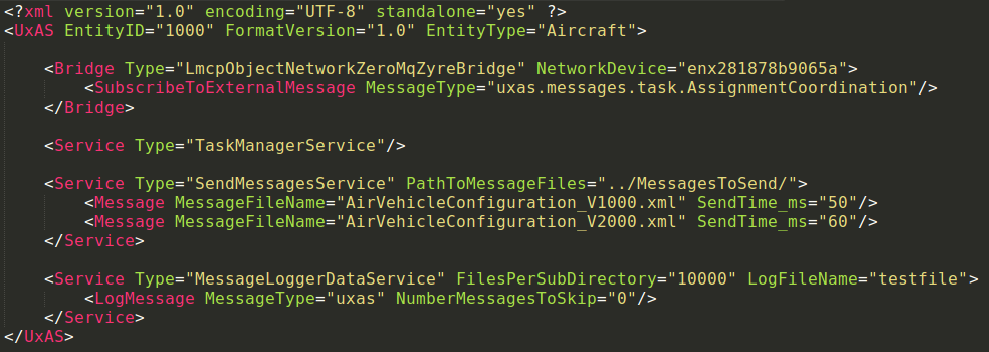
\includegraphics[width=1.3\linewidth]{\FiguresPath//ConfigExample}
	\caption{Sample configuration file}
	\label{fig:configExample}
\end{marginfigure}

Here is the \textbf{XML Declaration}:
\begin{docspec}<?xml version="1.0" encoding="UTF-8" standalone="yes" ?>\end{docspec}
The \textbf{UxAS Element}:
\begin{docspec}
	<UxAS EntityID="1000" FormatVersion="1.0" EntityType="Aircraft">
\end{docspec}
accepts the following attributes:
\begin{description}
	\item[\textit{EntityID}] Identification number of the entity represented by this instance of UxAS
	%\item[\textit{FormatVersion}] description ??????
	\item[\textit{EntityType}] used to differentiate between entities such as, \textit{Aircraft} and \textit{UGS}. Entries are defined by the services that use them.
	\item[\textit{ConsoleLoggerSeverityLevel}] if this attribute is present, all log messages at or below the severity level are displayed in the console. Valid entries are: \textit{DEBUG}, \textit{INFO}, \textit{WARN}, and \textit{ERROR}
	\item[\textit{MainFileLoggerSeverityLevel}] if this attribute is present, all log messages at or below the severity level are save in log files. Valid entries are: \textit{DEBUG}, \textit{INFO}, \textit{WARN}, and \textit{ERROR}
	%\item[\textit{StartDelay\_ms}] description
	\item[\textit{RunDuration\_s}] UxAS will run for \textit{RunDuration\_s} seconds before terminating.
	%\item[\textit{isLoggingThreadId}] description
\end{description}
Service Elements configure the services. There can be as many Service Elements as required. The attributes of the Service Elements are the options defined by each service. For example, the HelloWorld service can be configured with the following Service Element:
\begin{docspec}
	<Service Type="HelloWorld" StringToSend="Hello from \#1" SendPeriod\_ms="1000"/>
\end{docspec}
Bridge Elements configure bridges, which are services that create communication connections. For the Distributed Cooperation example, the zyre connection is configured with the following Bridge Element:
\begin{docspec}
    <Bridge Type="LmcpObjectNetworkZeroMqZyreBridge" NetworkDevice="enx281878b9065a">
	\quad<SubscribeToExternalMessage MessageType="uxas.messages.task.AssignmentCoordination"/>
	</Bridge>
\end{docspec}



\section{Core Services}\label{core-services}

The core services of UxAS work in concert to carry out the \emph{task assignment pipeline}
which automates the calculation of the proper vehicle-task orderings for efficient overall
mission completion. The design choice to seperate each of these services is motivated by
consideration of computational complexity as well as availability in the literature for
parts of the process (i.e. route planners and task assignment algorithms).

\begin{figure*}
	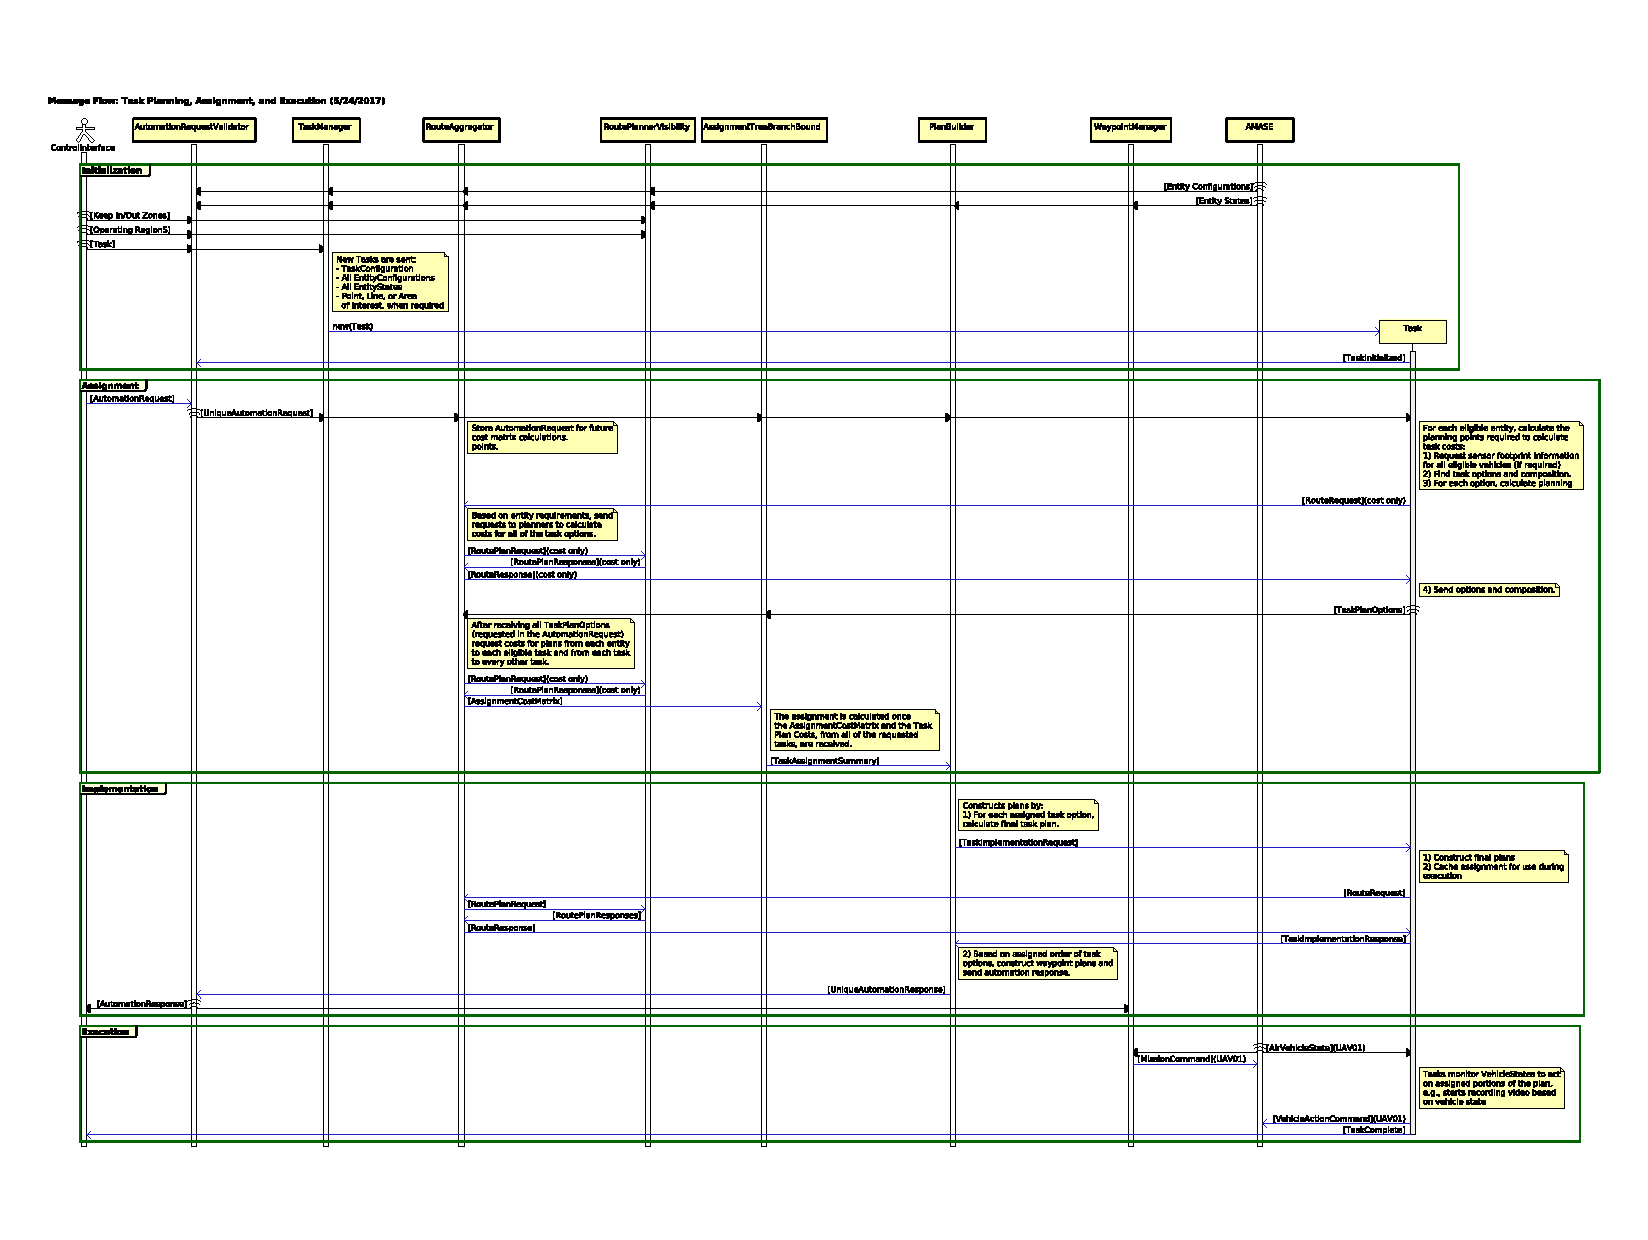
\includegraphics[width=1.0\linewidth]{\CCAFiguresPath//CCA_Components_MessageFLow}
	\caption{Message Flow for Task Assignment Pipeline}
	\label{fig:CoreServiceMessageFlow}
\end{figure*}

The message flow between the core services is captured in Figure~\ref{fig:CoreServiceMessageFlow}
and indicates the temporal relationship between the core services in carrying out a complete
automation request. Time proceeds from the top of the diagram to the bottom with
each horizontal arrow representing a single LMCP message of the specified type.

\begin{description}
\item
  \textbf{\textit{AutomationRequestValidatorService}} - This service will check an outside
  automation request for feasibility. If any task, vehicle, or operating region in the request
  has not yet been described to the system, this service will return an error indicating that
  the request cannot be fulfilled. If all necessary parts of the request are available to the
  system, then this service will attach a unique identifier to the request and start the
  sequence of steps necessary to fulfill that request. If any other outside requests are made
  while the system is in the process of fulfilling an existing request, this service will queue
  those additional requests, ensuring that the system only handles one request at a time. 
\item
  \textbf{\textit{TaskManagerService}} - This service dynamically creates new task services as
  their descriptions are sent into the system. When a new \textit{Task} is described, this service
  will send the proper configuration message for construction of a new service that adheres to
  the general task interface specification for that particular \textit{Task}. As part of the task
  service construction, this service will pass along all relevant details that a \textit{Task}
  needs for calculation of its behavior (i.e. current vehicle states, defined areas of interest, etc).
\item
  \textbf{\textit{Task}} - Tasks make up the atomic building blocks of automation requests. The
  composition of tasks and the assignment of particular vehicles to tasks comprises an automation
  response. When included as part of an automation request, a \textit{Task} reports a set of
  possible \emph{options} which represent the possible ways that the task can be completed. Each
  option is precisely a start and end location for applicable vehicles as well as the cost to
  complete the task using that option. The location and cost information for each option is used
  by the assignment service to select an option for each task that completes the overall mission
  efficiently. Once an option is selected by the assignment service, each \textit{Task} also
  reports the set of waypoints that a vehicle should use to complete the task.
\item
  \textbf{\textit{RoutePlannerVisibilityService}} - One of potentially many route planners, this
  service fulfills simple requests for routing in complex environments. For a given environment
  (described by sets of \textit{KeepIn} and \textit{KeepOut} polygons), a route planner will
  calculate the appropriate waypoints to guide a vehicle from a prescribed start location to a
  desired end location, ensuring that no waypoint is placed in an invalid area. This particular
  route planner uses a visibility graph as a basis to create distance-minimizing routes in two
  dimensions. Route planning services have a simple request-reply interface with each request
  corresponding to a single vehicle in a single environment.
\item
  \textbf{\textit{RouteAggregatorService}} - This service works with a set of route planners,
  requesting routes from the appropriate planner based on the situation. Additionally, this service
  provides the capability to make large-scale route planning requests involving multiple vehicles
  and multiple start/end locations. A primary use of this service is to calculate routes for all
  vehicles to travel between task locations. By orchestrating the cost-to-go calculations
  between tasks, this service acts as the bookkeeper for the complete cost map required by
  assignment algorithms.
\item
  \textbf{\textit{AssignmentTreeBranchBoundService}} - This service provides a resource allocation
  algorithm to determine an efficient use of the vehicle assets to fulfill tasks in the system. By
  design, the resource allocation is de-coupled from route planning and only uses the costs
  provided by the \textit{RouteAggregatorService}. The ultimate output of this service is an ordered
  list of tasks for each vehicle. This ordering must account for the process algebra relationship
  between tasks. This particular assignment service builds a tree of possible assignment orderings
  and prunes that tree based on the prescribed task relationships. The algorithm proceeds in two phases:
  1) greedy, depth-first search to find a feasible plan; 2) backtracking up the tree in a
  branch-and-bound manner to discover plans that are lower cost than the initial greedy plan. Once a
  predetermined amount of the tree has been searched (to ensure worst-case execution time), the
  assignment service will return the most efficient task ordering discovered.
\item
  \textbf{\textit{PlanBuilderService}} - With a task ordering determined by the assignment service,
  the \textit{PlanBuilderService} will organize the final set of waypoints that each vehicle should
  follow to complete the assignment. Working through the task ordering, this service requests the
  appropriate \textit{Tasks} in the assigned order to build a complete set of waypoints for each
  vehicle to carry out the mission. By stitching each part of the mission together in the proper
  order, this service provides the automation response that fulfills the original, outside
  automation request.
\end{description}

What follows are details for each of the core services and a rough description of the state machines
that each follows to complete its part of the overall task assignment process. See the auto-generated
LMCP documentation for precise details of each message.


%% use pandoc output of CoreServices.md `pandoc -o CoreServices.tex CoreServices.md`  %%
\subsection{AutomationRequestValidatorService}\label{automationrequestvalidatorservice}

This service provides a simple sanity check on external automation
requests. It also queues requests and tags them with unique identifiers,
feeding them into the system one at a time.

This service has two states: \textbf{idle} and \textbf{busy}. In both
states, when a non \emph{AutomationRequest} message is received, a local
memory store is updated to maintain a list of all available tasks,
vehicle configurations, vehicle states, zones, and operating regions.

Upon reception of an \emph{AutomationRequest} message, this service
ensures that such a request can be carried out by checking its local
memory store for existence of the requested vehicles, tasks, and
operating region. If the request includes vehicles, tasks, or an
operating region that has not previously been defined, this service will
publish an error message.

Upon determination that the \emph{AutomationRequest} includes only
vehicles, tasks, and an operating region that have previously been
defined, this service creates a \emph{UniqueAutomationRequest} with a
previously unused unique identifier. If in the \textbf{idle} state, this
service will immediately publish the \emph{UniqueAutomationRequest}
message and transition to the \textbf{busy} state. If already in the
\textbf{busy} state, the \emph{UniqueAutomationRequest} will be added to
the end of a queue.

When this service receives either an error message (indicating that the
\emph{UniqueAutomationRequest} cannot be fulfilled or a corresponding
\emph{UniqueAutomationResponse}), it will publish the same message. If
in the \textbf{idle} state, it will remain in the \textbf{idle} state.
If in the \textbf{busy} state, it will remove from the queue the request
that was just fulfilled and then send the next
\emph{UniqueAutomationRequest} in the queue. If the queue is empty, this
service transitions back to the \textbf{idle} state.

This service also includes a parameter that allows an optional
\emph{timeout} value to be set. When a \emph{UniqueAutomationRequest} is
published, a timer begins. If the \emph{timeout} has been reached before
a \emph{UniqueAutomationResponse} is received, an error is assumed to
have occured and this service removes the pending
\emph{UniqueAutomationRequest} from the queue and attempts to send the
next in the queue or transition to \textbf{idle} if the queue is empty.

\begin{longtable}[c]{@{}ll@{}}
\caption{Table of messages that the
\emph{AutomationRequestValidatorService} receives and
processes.}\tabularnewline
\toprule
\begin{minipage}[b]{0.29\columnwidth}\raggedright\strut
Message Subscription
\strut\end{minipage} &
\begin{minipage}[b]{0.65\columnwidth}\raggedright\strut
Description
\strut\end{minipage}\tabularnewline
\midrule
\endfirsthead
\toprule
\begin{minipage}[b]{0.29\columnwidth}\raggedright\strut
Message Subscription
\strut\end{minipage} &
\begin{minipage}[b]{0.65\columnwidth}\raggedright\strut
Description
\strut\end{minipage}\tabularnewline
\midrule
\endhead
\begin{minipage}[t]{0.29\columnwidth}\raggedright\strut
\emph{AutomationRequest}
\strut\end{minipage} &
\begin{minipage}[t]{0.65\columnwidth}\raggedright\strut
Primary message to request a set of Tasks to be completed by a set of
vehicles in a particular airspace configuration (described by an
\emph{OperatingRegion}).
\strut\end{minipage}\tabularnewline
\begin{minipage}[t]{0.29\columnwidth}\raggedright\strut
\emph{EntityConfiguration}
\strut\end{minipage} &
\begin{minipage}[t]{0.65\columnwidth}\raggedright\strut
Vehicle capabilities (e.g.~allowable speeds) are described by entity
configuration messages. Any vehicle requested in an
\emph{AutomationRequest} must previously be described by an associated
\emph{EntityConfiguration}.
\strut\end{minipage}\tabularnewline
\begin{minipage}[t]{0.29\columnwidth}\raggedright\strut
\emph{EntityState}
\strut\end{minipage} &
\begin{minipage}[t]{0.65\columnwidth}\raggedright\strut
Describes the actual state of a vehicle in the system including
position, speed, and fuel status. Each vehicle in an
\emph{AutomationRequest} must have reported its state.
\strut\end{minipage}\tabularnewline
\begin{minipage}[t]{0.29\columnwidth}\raggedright\strut
\emph{Task}
\strut\end{minipage} &
\begin{minipage}[t]{0.65\columnwidth}\raggedright\strut
Details a particular task that will be referenced (by ID) in an
\emph{AutomationRequest}.
\strut\end{minipage}\tabularnewline
\begin{minipage}[t]{0.29\columnwidth}\raggedright\strut
\emph{TaskInitialized}
\strut\end{minipage} &
\begin{minipage}[t]{0.65\columnwidth}\raggedright\strut
Indicates that a particular task is ready to proceed with the task
assignment sequence. Each task requested in the \emph{AutomationRequest}
must be initialized before a \emph{UniqueAutomationRequest} is
published.
\strut\end{minipage}\tabularnewline
\begin{minipage}[t]{0.29\columnwidth}\raggedright\strut
\emph{KeepOutZone}
\strut\end{minipage} &
\begin{minipage}[t]{0.65\columnwidth}\raggedright\strut
Polygon description of a region in which vehicles must not travel. If
referenced by the \emph{OperatingRegion} in the
\emph{AutomationRequest}, zone must exist for request to be valid.
\strut\end{minipage}\tabularnewline
\begin{minipage}[t]{0.29\columnwidth}\raggedright\strut
\emph{KeepInZone}
\strut\end{minipage} &
\begin{minipage}[t]{0.65\columnwidth}\raggedright\strut
Polygon description of a region in which vehicles must remain during
travel. If referenced by the \emph{OperatingRegion} in the
\emph{AutomationRequest}, zone must exist for request to be valid.
\strut\end{minipage}\tabularnewline
\begin{minipage}[t]{0.29\columnwidth}\raggedright\strut
\emph{OperatingRegion}
\strut\end{minipage} &
\begin{minipage}[t]{0.65\columnwidth}\raggedright\strut
Collection of \emph{KeepIn} and \emph{KeepOut} zones that describe the
allowable space for vehicular travel. Must be defined for
\emph{AutomationRequest} to be valid.
\strut\end{minipage}\tabularnewline
\begin{minipage}[t]{0.29\columnwidth}\raggedright\strut
\emph{UniqueAutomationResponse}
\strut\end{minipage} &
\begin{minipage}[t]{0.65\columnwidth}\raggedright\strut
Completed response from the rest of the task assignment process.
Indicates that the next \emph{AutomationRequest} is ready to be
processed.
\strut\end{minipage}\tabularnewline
\bottomrule
\end{longtable}

\begin{longtable}[c]{@{}ll@{}}
\caption{Table of messages that the
\emph{AutomationRequestValidatorService} publishes.}\tabularnewline
\toprule
\begin{minipage}[b]{0.29\columnwidth}\raggedright\strut
Message Publication
\strut\end{minipage} &
\begin{minipage}[b]{0.65\columnwidth}\raggedright\strut
Description
\strut\end{minipage}\tabularnewline
\midrule
\endfirsthead
\toprule
\begin{minipage}[b]{0.29\columnwidth}\raggedright\strut
Message Publication
\strut\end{minipage} &
\begin{minipage}[b]{0.65\columnwidth}\raggedright\strut
Description
\strut\end{minipage}\tabularnewline
\midrule
\endhead
\begin{minipage}[t]{0.29\columnwidth}\raggedright\strut
\emph{UniqueAutomationRequest}
\strut\end{minipage} &
\begin{minipage}[t]{0.65\columnwidth}\raggedright\strut
A duplicate message to an external \emph{AutomationRequest} but only
published if the request is determined to be valid. Also includes a
unique identifier to match to the corresponding response.
\strut\end{minipage}\tabularnewline
\begin{minipage}[t]{0.29\columnwidth}\raggedright\strut
\emph{ServiceStatus}
\strut\end{minipage} &
\begin{minipage}[t]{0.65\columnwidth}\raggedright\strut
Error message when a request is determined to be invalid. Includes human
readable error message that highlights which portion of the
\emph{AutomationRequest} was invalid.
\strut\end{minipage}\tabularnewline
\begin{minipage}[t]{0.29\columnwidth}\raggedright\strut
\emph{AutomationResponse}
\strut\end{minipage} &
\begin{minipage}[t]{0.65\columnwidth}\raggedright\strut
Upon reception of a completed \emph{UniqueAutomationResponse}, this
message is published as a response to the original request.
\strut\end{minipage}\tabularnewline
\bottomrule
\end{longtable}

\subsection{TaskManagerService}\label{taskmanagerservice}

The \emph{TaskManagerService} is a very straight-forward service. Upon
reception of a Task message, it will send the appropriate
\emph{CreateNewService} message. To do so, it catalogues all entity
configurations and current states; areas, lines, and points of interest;
and current waypoint paths for each vehicle. This information is stored
in local memory and appended as part of the \emph{CreateNewService}
message which allows new Tasks to immediately be informed of all
relevant information needed to carry out a Task.

When \emph{TaskManagerService} receives a \emph{RemoveTasks} message, it
will form the appropriate \emph{KillService} message to properly destroy
the service that was created to fulfill the original Task.

\begin{longtable}[c]{@{}ll@{}}
\caption{Table of messages that the \emph{TaskManagerService} receives
and processes.}\tabularnewline
\toprule
\begin{minipage}[b]{0.29\columnwidth}\raggedright\strut
Message Subscription
\strut\end{minipage} &
\begin{minipage}[b]{0.65\columnwidth}\raggedright\strut
Description
\strut\end{minipage}\tabularnewline
\midrule
\endfirsthead
\toprule
\begin{minipage}[b]{0.29\columnwidth}\raggedright\strut
Message Subscription
\strut\end{minipage} &
\begin{minipage}[b]{0.65\columnwidth}\raggedright\strut
Description
\strut\end{minipage}\tabularnewline
\midrule
\endhead
\begin{minipage}[t]{0.29\columnwidth}\raggedright\strut
\emph{Task}
\strut\end{minipage} &
\begin{minipage}[t]{0.65\columnwidth}\raggedright\strut
Primary message that describes a particular task. The task manager will
make the appropriate service creation message to build a service that
directly handles this requested Task.
\strut\end{minipage}\tabularnewline
\begin{minipage}[t]{0.29\columnwidth}\raggedright\strut
\emph{RemoveTasks}
\strut\end{minipage} &
\begin{minipage}[t]{0.65\columnwidth}\raggedright\strut
Indicates that Task is no longer needed and will not be included in
future \emph{AutomationRequest} messages. Task manager will send the
proper \emph{KillService} message to remove the service that was
constructed to handle the requested Task.
\strut\end{minipage}\tabularnewline
\begin{minipage}[t]{0.29\columnwidth}\raggedright\strut
\emph{EntityConfiguration}
\strut\end{minipage} &
\begin{minipage}[t]{0.65\columnwidth}\raggedright\strut
Vehicle capabilities (e.g.~allowable speeds) are described by entity
configuration messages. New Tasks are informed of all known entities
upon creation.
\strut\end{minipage}\tabularnewline
\begin{minipage}[t]{0.29\columnwidth}\raggedright\strut
\emph{EntityState}
\strut\end{minipage} &
\begin{minipage}[t]{0.65\columnwidth}\raggedright\strut
Describes the actual state of a vehicle in the system including
position, speed, and fuel status. New Tasks are informed of all known
entity states upon creation.
\strut\end{minipage}\tabularnewline
\begin{minipage}[t]{0.29\columnwidth}\raggedright\strut
\emph{AreaOfInterest} \emph{LineOfInterest} \emph{PointOfInterest}
\strut\end{minipage} &
\begin{minipage}[t]{0.65\columnwidth}\raggedright\strut
Describes known geometries of areas, lines, and points. New Tasks are
informed of all such named areas upon creation.
\strut\end{minipage}\tabularnewline
\begin{minipage}[t]{0.29\columnwidth}\raggedright\strut
\emph{MissionCommand}
\strut\end{minipage} &
\begin{minipage}[t]{0.65\columnwidth}\raggedright\strut
Describes current set of waypoints that a vehicle is following. New
Tasks are informed of all known current waypoint routes upon creation.
\strut\end{minipage}\tabularnewline
\bottomrule
\end{longtable}

\begin{longtable}[c]{@{}ll@{}}
\caption{Table of messages that the \emph{TaskManagerService}
publishes.}\tabularnewline
\toprule
\begin{minipage}[b]{0.29\columnwidth}\raggedright\strut
Message Publication
\strut\end{minipage} &
\begin{minipage}[b]{0.65\columnwidth}\raggedright\strut
Description
\strut\end{minipage}\tabularnewline
\midrule
\endfirsthead
\toprule
\begin{minipage}[b]{0.29\columnwidth}\raggedright\strut
Message Publication
\strut\end{minipage} &
\begin{minipage}[b]{0.65\columnwidth}\raggedright\strut
Description
\strut\end{minipage}\tabularnewline
\midrule
\endhead
\begin{minipage}[t]{0.29\columnwidth}\raggedright\strut
\emph{CreateNewService}
\strut\end{minipage} &
\begin{minipage}[t]{0.65\columnwidth}\raggedright\strut
Primary message published by the Task Manager to dynamically build a new
Task from an outside description of such a Task.
\strut\end{minipage}\tabularnewline
\begin{minipage}[t]{0.29\columnwidth}\raggedright\strut
\emph{KillService}
\strut\end{minipage} &
\begin{minipage}[t]{0.65\columnwidth}\raggedright\strut
When Tasks are no longer needed, the Task Manager will correctly clean
up and destroy the service that was built to handle the original Task.
\strut\end{minipage}\tabularnewline
\bottomrule
\end{longtable}

\subsection{Task}\label{task}

A \emph{Task} forms the core functionality of vehicle behavior. It is
the point at which a vehicle (or set of vehicles) is dedicated to a
singular goal. During \emph{Task} execution, a wide spectrum of behavior
is allowed, including updating waypoints and steering sensors. As part
of the core services, this general \emph{Task} description stands in for
all \emph{Tasks} running in the system.

The general \emph{Task} interaction with the rest of the task assignment
pipeline is complex. It is the aggregation of each \emph{Task's}
possibilities that defines the complexity of the overall mission
assignment. These \emph{Task} possibilities are called \emph{options}
and they describe the precise ways that a \emph{Task} could unfold. For
example, a \emph{LineSearchTask} could present two options to the
system: 1) search the line from East-to-West and 2) search the line from
West-to-East. Either is valid and a selection of one of these options
that optimizes overall mission efficiency is the role of the assignment
service.

A general \emph{Task} is comprised of up to nine states with each state
corresponding to a place in the message sequence that carries out the
task assignment pipeline. The states for a \emph{Task} are:

\begin{itemize}
\tightlist
\item
  \textbf{Init}: This is the state that all \emph{Tasks} start in and
  remain until all internal initialization is complete. For example, a
  \emph{Task} may need to load complex terrain or weather data upon
  creation and will require some (possibly significant) start-up time.
  When a \emph{Task} has completed its internal initialization, it must
  report transition from this state via the \emph{TaskInitialized}
  message.
\item
  \textbf{Idle}: This represents the state of a \emph{Task} after
  initialization, but before any requests have been made that include
  the \emph{Task}. \emph{UniqueAutomationRequest} messages trigger a
  transition from this state into the \textbf{SensorRequest} state.
\item
  \textbf{SensorRequest}: When a \emph{Task} is notified of its
  inclusion (by noting the presence of its ID in the \emph{Tasks} list
  of an \emph{UniqueAutomationRequest} message), it can request
  calculations that pertain to the sensors onboard the vehicles that are
  also included in the \emph{UniqueAutomationRequest} message. While
  waiting for a response from the \emph{SensorManagerService}, a
  \emph{Task} is in the \textbf{SensorRequest} state and will remain so
  until the response from the \emph{SensorManagerService} is received.
\item
  \textbf{OptionRoutes}: After the \emph{SensorManagerService} has
  replied with the appropriate sensor calculations, the \emph{Task} can
  request waypoints from the \emph{RouteAggregatorService} that carry
  out the on-\emph{Task} goals. For example, an \emph{AreaSearchTask}
  can request routes from key surveillance positions that ensure sensor
  coverage of the entire area. The \emph{Task} remains in the
  \textbf{OptionRoutes} state until the \emph{RouteAggregatorService}
  replies.
\item
  \textbf{OptionsPublished}: When routes are returned to the
  \emph{Task}, it will utilize all route and sensor information to
  identify and publish the applicable \emph{TaskOptions}. The
  determination of \emph{TaskOptions} is key to overall mission
  performance and vehicle behavior. It is from this list of options that
  the assignment will select in order to perform this particular
  \emph{Task}. After publication of the options, a \emph{Task} waits in
  the \textbf{OptionsPublished} state until the
  \emph{TaskImplementationRequest} message is received, whereupon it
  switches to \textbf{FinalRoutes}.
\item
  \textbf{FinalRoutes}: Upon reception of a
  \emph{TaskImplementationRequest}, a \emph{Task} is informed of the
  option that was selected by the assignment service. At this point, a
  \emph{Task} must create the final set of waypoints that include both
  \emph{enroute} and \emph{on-task} waypoints from the specified vehicle
  location. The \emph{Task} is required to create the \emph{enroute}
  waypoints since a route refinement is possible, taking advantage of
  the concrete prior position of the selected vehicle. The \emph{Task}
  remains in the \textbf{FinalRoutes} state until the route request is
  fulfilled by the \emph{RouteAggregatorService}.
\item
  \textbf{OptionSelected}: When the final waypoints are returned from
  the \emph{RouteAggregatorService}, the \emph{Task} publishes a
  complete \emph{TaskImplementationResponse} message. A \emph{Task} will
  remain in this state until an \emph{EntityState} message includes this
  \emph{Task} ID in its \emph{AssociatedTaskList}. If during this state,
  a subsequent \emph{UniqueAutomationRequest} is made, the \emph{Task}
  returns to the \textbf{SensorRequest} state and immediately attempts
  to fulfill the requirements of the new \emph{UniqueAutomationRequest}.
  This behavior implies that a \emph{Task} can only be part of a single
  \emph{AutomationRequest} and subsequent requests always override
  previous requests.
\item
  \textbf{Active}: If the \emph{Task} is in the \textbf{OptionSelected}
  state and an \emph{EntityState} message is received which includes the
  \emph{Task} ID in the \emph{AssociatedTaskList}, then the \emph{Task}
  switches to the \textbf{Active} state and is allowed to publish new
  waypoints and sensor commands at will. A \emph{Task} remains in the
  \textbf{Active} state until a subsequent \emph{EntityState} message
  does \emph{not} list the \emph{Task} ID in its
  \emph{AssociatedTaskList}. At which point, a transition to
  \textbf{Completed} is made. Note that a \emph{Task} can reliquish
  control indirectly by sending the vehicle to a waypoint not tagged
  with its own ID. Likewise, it can maintain control indefinitely by
  ensuring that the vehicle only ever go to a waypoint that includes its
  ID. If a \emph{UniqueAutomationRequest} message that includes this
  \emph{Task} ID is received in the \textbf{Active} state, it
  transitions to the \textbf{Completed} state.
\item
  \textbf{Completed}: In this state, the \emph{Task} publishes a
  \emph{TaskComplete} message and then immediately transitions to the
  \textbf{Idle} state.
\end{itemize}

\begin{longtable}[c]{@{}ll@{}}
\caption{Table of messages that a general \emph{Task} receives and
processes.}\tabularnewline
\toprule
\begin{minipage}[b]{0.29\columnwidth}\raggedright\strut
Message Subscription
\strut\end{minipage} &
\begin{minipage}[b]{0.65\columnwidth}\raggedright\strut
Description
\strut\end{minipage}\tabularnewline
\midrule
\endfirsthead
\toprule
\begin{minipage}[b]{0.29\columnwidth}\raggedright\strut
Message Subscription
\strut\end{minipage} &
\begin{minipage}[b]{0.65\columnwidth}\raggedright\strut
Description
\strut\end{minipage}\tabularnewline
\midrule
\endhead
\begin{minipage}[t]{0.29\columnwidth}\raggedright\strut
\emph{UniqueAutomationRequest}
\strut\end{minipage} &
\begin{minipage}[t]{0.65\columnwidth}\raggedright\strut
Indicates which \emph{Tasks} are to be considered as well as the set of
vehicles that can be used to fulfill those \emph{Tasks}. Upon reception
of this message, if a \emph{Task} ID is included, it will publish
\emph{TaskPlanOptions}.
\strut\end{minipage}\tabularnewline
\begin{minipage}[t]{0.29\columnwidth}\raggedright\strut
\emph{TaskImplementationRequest}
\strut\end{minipage} &
\begin{minipage}[t]{0.65\columnwidth}\raggedright\strut
After an assignment has been made, each \emph{Task} involved is
requested to build the final set of waypoints that complete the
\emph{Task} and corresponding selected option. A \emph{Task} must build
the route \textbf{to} the \emph{Task} as well as waypoints that
implement the \emph{Task}. For each on-task waypoint, the
\emph{AssociatedTaskList} must include the \emph{Task} ID.
\strut\end{minipage}\tabularnewline
\begin{minipage}[t]{0.29\columnwidth}\raggedright\strut
\emph{EntityConfiguration}
\strut\end{minipage} &
\begin{minipage}[t]{0.65\columnwidth}\raggedright\strut
Vehicle capabilities (e.g.~allowable speeds) are described by entity
configuration messages. \emph{Tasks} can reason over sensor and vehicle
capabilites to present the proper options to other parts of the system.
If a vehicle does not have the capability to fulfill the \emph{Task}
(e.g.~does not have a proper sensor), then the \emph{Task} shall not
include that vehicle ID in the list of eligible entities reported as
part of an option.
\strut\end{minipage}\tabularnewline
\begin{minipage}[t]{0.29\columnwidth}\raggedright\strut
\emph{EntityState}
\strut\end{minipage} &
\begin{minipage}[t]{0.65\columnwidth}\raggedright\strut
Describes the actual state of a vehicle in the system including
position, speed, and fuel status. This message is primary feedback
mechanism used for \emph{Tasks} to switch to an \textbf{Active} state.
When a \emph{Task} ID is listed in the \emph{AssociatedTaskList} of an
\emph{EntityState} message, the \emph{Task} is allowed to update
waypoints and sensor commands at will.
\strut\end{minipage}\tabularnewline
\begin{minipage}[t]{0.29\columnwidth}\raggedright\strut
\emph{RouteResponse}
\strut\end{minipage} &
\begin{minipage}[t]{0.65\columnwidth}\raggedright\strut
Collection of route plans that fulfill a set of requests for navigation
through an \emph{OperatingRegion}. A \emph{Task} must request the
waypoints to route a vehicle from its last to the start of the
\emph{Task}. Additionally, this message can be used to obtain on-task
waypoints.
\strut\end{minipage}\tabularnewline
\bottomrule
\end{longtable}

\begin{longtable}[c]{@{}ll@{}}
\caption{Table of messages that a general \emph{Task}
publishes.}\tabularnewline
\toprule
\begin{minipage}[b]{0.29\columnwidth}\raggedright\strut
Message Publication
\strut\end{minipage} &
\begin{minipage}[b]{0.65\columnwidth}\raggedright\strut
Description
\strut\end{minipage}\tabularnewline
\midrule
\endfirsthead
\toprule
\begin{minipage}[b]{0.29\columnwidth}\raggedright\strut
Message Publication
\strut\end{minipage} &
\begin{minipage}[b]{0.65\columnwidth}\raggedright\strut
Description
\strut\end{minipage}\tabularnewline
\midrule
\endhead
\begin{minipage}[t]{0.29\columnwidth}\raggedright\strut
\emph{TaskPlanOptions}
\strut\end{minipage} &
\begin{minipage}[t]{0.65\columnwidth}\raggedright\strut
Primary message published by a \emph{Task} to indicate the potential
different ways a \emph{Task} could be completed. Each possible way to
fulfill a \emph{Task} is listed as an \emph{option}. \emph{TaskOptions}
can also be related to each other via Process Algebra.
\strut\end{minipage}\tabularnewline
\begin{minipage}[t]{0.29\columnwidth}\raggedright\strut
\emph{TaskImplementationResponse}
\strut\end{minipage} &
\begin{minipage}[t]{0.65\columnwidth}\raggedright\strut
Primary message published by a \emph{Task} that reports the final set of
waypoints to both navigate the selected vehicle to the \emph{Task} as
well as the waypoints necessary to complete the \emph{Task} using the
selected option.
\strut\end{minipage}\tabularnewline
\begin{minipage}[t]{0.29\columnwidth}\raggedright\strut
\emph{RouteRequest}
\strut\end{minipage} &
\begin{minipage}[t]{0.65\columnwidth}\raggedright\strut
Collection of route plan requests to leverage the route planner
capability of constructing waypoints that adhere to the designated
\emph{OperatingRegion}. This request is made for waypoints en-route to
the \emph{Task} as well as on-task waypoints.
\strut\end{minipage}\tabularnewline
\begin{minipage}[t]{0.29\columnwidth}\raggedright\strut
\emph{VehicleActionCommand}
\strut\end{minipage} &
\begin{minipage}[t]{0.65\columnwidth}\raggedright\strut
When a \emph{Task} is \textbf{Active}, it is allowed to update sensor
navigation commands to on-task vehicles. This message is used to
directly command the vehicle to use the updated behaviors calculated by
the \emph{Task}.
\strut\end{minipage}\tabularnewline
\begin{minipage}[t]{0.29\columnwidth}\raggedright\strut
\emph{TaskComplete}
\strut\end{minipage} &
\begin{minipage}[t]{0.65\columnwidth}\raggedright\strut
Once a \emph{Task} has met its goal or if a vehicle reports that it is
no longer on-task, a previously \textbf{Active} \emph{Task} must send a
\emph{TaskComplete} message to inform the system of this change.
\strut\end{minipage}\tabularnewline
\bottomrule
\end{longtable}

\subsection{RoutePlannerVisibilityService}\label{routeplannervisibilityservice}

The \emph{RoutePlannerVisibilityService} is a service that provides
route planning using a visibility heuristic. One of the fundamental
architectural decisions in UxAS is separation of route planning from
task assignment. This service is an example of a route planning service
for aircraft. Ground vehicle route planning (based on Open Street Maps
data) can be found in the \emph{OsmPlannerService}.

The design of the \emph{RoutePlannerVisibilityService} message interface
is intended to be as simple as possible: a route planning service
considers routes only in fixed environments for known vehicles and
handles requests for single vehicles. The logic necessary to plan for
multiple (possibly heterogeneous) vehicles is handled in the
\emph{RouteAggregatorService}.

In two dimensional environments composed of polygons, the shortest
distance between points lies on the visibility graph. The
\emph{RoutePlannerVisibilityService} creates such a graph and, upon
request, adds desired start/end locations to quickly approximate a
distance-optimal route through the environment. With the straight-line
route created by the searching the visibility graph, a smoothing
operation is applied to ensure that minimum turn rate constraints of
vehicles are satisfied. Note, this smoothing operation can violate the
prescribed keep-out zones and is not guaranteed to smooth arbitrary
straight-line routes (in particular, path segments shorter than the
minimum turn radius can be problematic).

Due to the need to search over many possible orderings of \emph{Tasks}
during an assignment calculation, the route planner must very quickly
compute routes. Even for small problems, hundreds of routes must be
calculated before the assignment algorithm can start searching over the
possible ordering. For this reason it is imperative that the route
planner be responsive and efficient.

\begin{longtable}[c]{@{}ll@{}}
\caption{Table of messages that the \emph{RoutePlannerVisibilityService}
receives and processes.}\tabularnewline
\toprule
\begin{minipage}[b]{0.29\columnwidth}\raggedright\strut
Message Subscription
\strut\end{minipage} &
\begin{minipage}[b]{0.65\columnwidth}\raggedright\strut
Description
\strut\end{minipage}\tabularnewline
\midrule
\endfirsthead
\toprule
\begin{minipage}[b]{0.29\columnwidth}\raggedright\strut
Message Subscription
\strut\end{minipage} &
\begin{minipage}[b]{0.65\columnwidth}\raggedright\strut
Description
\strut\end{minipage}\tabularnewline
\midrule
\endhead
\begin{minipage}[t]{0.29\columnwidth}\raggedright\strut
\emph{RoutePlanRequest}
\strut\end{minipage} &
\begin{minipage}[t]{0.65\columnwidth}\raggedright\strut
Primary message that describes a route plan request. A request considers
only a single vehicle in a single \emph{OperatingRegion} although it can
request multiple pairs of start and end locations with a single message.
\strut\end{minipage}\tabularnewline
\begin{minipage}[t]{0.29\columnwidth}\raggedright\strut
\emph{KeepOutZone}
\strut\end{minipage} &
\begin{minipage}[t]{0.65\columnwidth}\raggedright\strut
Polygon description of a region in which vehicles must not travel. This
service will track all \emph{KeepOutZones} to compose them upon
reception of an \emph{OperatingRegion}.
\strut\end{minipage}\tabularnewline
\begin{minipage}[t]{0.29\columnwidth}\raggedright\strut
\emph{KeepInZone}
\strut\end{minipage} &
\begin{minipage}[t]{0.65\columnwidth}\raggedright\strut
Polygon description of a region in which vehicles must remain during
travel. This service will track all \emph{KeepInZones} to compose them
upon reception of an \emph{OperatingRegion}.
\strut\end{minipage}\tabularnewline
\begin{minipage}[t]{0.29\columnwidth}\raggedright\strut
\emph{OperatingRegion}
\strut\end{minipage} &
\begin{minipage}[t]{0.65\columnwidth}\raggedright\strut
Collection of \emph{KeepIn} and \emph{KeepOut} zones that describe the
allowable space for vehicular travel. When received, this service
creates a visibility graph considering the zones referenced by this
\emph{OperatingRegion}. Upon \emph{RoutePlanRequest} the visibility
graph corresponding to the \emph{OperatingRegion} ID is retreived and
manipulated to add start/end locations and perform the shortest path
search.
\strut\end{minipage}\tabularnewline
\begin{minipage}[t]{0.29\columnwidth}\raggedright\strut
\emph{EntityConfiguration}
\strut\end{minipage} &
\begin{minipage}[t]{0.65\columnwidth}\raggedright\strut
Vehicle capabilities (e.g.~allowable speeds) are described by entity
configuration messages. This service calculates the minimum turn radius
of the entity by using the max bank angle and nominal speed. Requested
routes are then returned at the nominal speed and with turns
approximating the minimum turn radius.
\strut\end{minipage}\tabularnewline
\begin{minipage}[t]{0.29\columnwidth}\raggedright\strut
``AircraftPathPlanner''
\strut\end{minipage} &
\begin{minipage}[t]{0.65\columnwidth}\raggedright\strut
In addition to subscribing to the above broadcasted messages, this
service also subscribes to the group mailbox for path planners that
service aircraft requests. Upon reception of a message on this channel,
the service will check for one of the above messages and process it as
if it came from over the broadcast channel. In either case, the return
message always uses return-to-sender addressing.
\strut\end{minipage}\tabularnewline
\bottomrule
\end{longtable}

\begin{longtable}[c]{@{}ll@{}}
\caption{Table of messages that the \emph{RoutePlannerVisibilityService}
publishes.}\tabularnewline
\toprule
\begin{minipage}[b]{0.29\columnwidth}\raggedright\strut
Message Publication
\strut\end{minipage} &
\begin{minipage}[b]{0.65\columnwidth}\raggedright\strut
Description
\strut\end{minipage}\tabularnewline
\midrule
\endfirsthead
\toprule
\begin{minipage}[b]{0.29\columnwidth}\raggedright\strut
Message Publication
\strut\end{minipage} &
\begin{minipage}[b]{0.65\columnwidth}\raggedright\strut
Description
\strut\end{minipage}\tabularnewline
\midrule
\endhead
\begin{minipage}[t]{0.29\columnwidth}\raggedright\strut
\emph{RoutePlanResponse}
\strut\end{minipage} &
\begin{minipage}[t]{0.65\columnwidth}\raggedright\strut
This message contains the waypoints and time cost that fulfills the
route request. This message is the only one published by the
\emph{RoutePlannerVisibilityService} and is always sent using the
return-to-sender addressing which ensures that only the original
requester receives the response.
\strut\end{minipage}\tabularnewline
\bottomrule
\end{longtable}

\subsection{RouteAggregatorService}\label{routeaggregatorservice}

The \emph{RouteAggregatorService} fills two primary roles: 1) it acts as
a helper service to make route requests for large numbers of
heterogenous vehicles; and 2) it constructs the task-to-task route-cost
table that is used by the assignment service to order the tasks as
efficiently as possible. Each functional role acts independently and can
be modeled as two different state machines.

The \emph{Aggregator} role orchestrates large numbers of route requests
(possibly to multiple route planners). This allows other services in the
system (such as \emph{Tasks}) to make a single request for routes and
receive a single reply with the complete set of routes for numerous
vehicles.

For every aggregate route request (specified by a \emph{RouteRequest}
message), the \emph{Aggregator} makes a series of
\emph{RoutePlanRequests} to the appropriate route planners (i.e.~sending
route plan requests for ground vehicles to the ground vehicle planner
and route plan requests for aircraft to the aircraft planner). Each
request is marked with a request ID and a list of all request IDs that
must have matching replies is created. The \emph{Aggregator} then enters
a \textbf{pending} state in which all received plan replies are stored
and then checked off the list of expected replies. When all of the
expected replies have been received, the \emph{Aggregator} publishes the
completed \emph{RouteResponse} and returns to the \textbf{idle} state.

Note that every aggregate route request corresponds to a separate
internal checklist of expected responses that will fulfill the original
aggregate request. The \emph{Aggregator} is designed to service each
aggregate route request even if a previous one is in the process of
being fulfilled. When the \emph{Aggregator} receives any response from a
route planner, it checks each of the many checklists to determine if all
expected responses for a particuarl list have been met. In this way, the
\emph{Aggregator} is in a different \textbf{pending} state for each
aggregate request made to it.

\begin{longtable}[c]{@{}ll@{}}
\caption{Table of messages that the \emph{RouteAggregatorService}
receives and processes in its \emph{Aggregator} role.}\tabularnewline
\toprule
\begin{minipage}[b]{0.29\columnwidth}\raggedright\strut
Message Subscription
\strut\end{minipage} &
\begin{minipage}[b]{0.65\columnwidth}\raggedright\strut
Description
\strut\end{minipage}\tabularnewline
\midrule
\endfirsthead
\toprule
\begin{minipage}[b]{0.29\columnwidth}\raggedright\strut
Message Subscription
\strut\end{minipage} &
\begin{minipage}[b]{0.65\columnwidth}\raggedright\strut
Description
\strut\end{minipage}\tabularnewline
\midrule
\endhead
\begin{minipage}[t]{0.29\columnwidth}\raggedright\strut
\emph{RouteRequest}
\strut\end{minipage} &
\begin{minipage}[t]{0.65\columnwidth}\raggedright\strut
Primary message that requests a large number of routes for potentially
heterogeneous vehicles. The \emph{Aggregator} will make a series of
\emph{RoutePlanRequests} to the appropriate planners to fulfill this
request.
\strut\end{minipage}\tabularnewline
\begin{minipage}[t]{0.29\columnwidth}\raggedright\strut
\emph{EntityConfiguration}
\strut\end{minipage} &
\begin{minipage}[t]{0.65\columnwidth}\raggedright\strut
Vehicle capabilities (e.g.~allowable speeds) are described by entity
configuration messages. This service uses the \emph{EntityConfiguration}
to determine which type of vehicle corresponds to a specific ID so that
ground planners are used for ground vehicles and air planners are used
for aircraft.
\strut\end{minipage}\tabularnewline
\begin{minipage}[t]{0.29\columnwidth}\raggedright\strut
\emph{RoutePlanResponse}
\strut\end{minipage} &
\begin{minipage}[t]{0.65\columnwidth}\raggedright\strut
This message is the fulfillment of a single vehicle route plan request
which the \emph{Aggregator} catalogues until the complete set of
expected responses is received.
\strut\end{minipage}\tabularnewline
\bottomrule
\end{longtable}

\begin{longtable}[c]{@{}ll@{}}
\caption{Table of messages that the \emph{RouteAggregatorService}
publishes in its \emph{Aggregator} role.}\tabularnewline
\toprule
\begin{minipage}[b]{0.29\columnwidth}\raggedright\strut
Message Publication
\strut\end{minipage} &
\begin{minipage}[b]{0.65\columnwidth}\raggedright\strut
Description
\strut\end{minipage}\tabularnewline
\midrule
\endfirsthead
\toprule
\begin{minipage}[b]{0.29\columnwidth}\raggedright\strut
Message Publication
\strut\end{minipage} &
\begin{minipage}[b]{0.65\columnwidth}\raggedright\strut
Description
\strut\end{minipage}\tabularnewline
\midrule
\endhead
\begin{minipage}[t]{0.29\columnwidth}\raggedright\strut
\emph{RouteResponse}
\strut\end{minipage} &
\begin{minipage}[t]{0.65\columnwidth}\raggedright\strut
Once the \emph{Aggregator} has a complete set of responses collected
from the route planners, the message is built as a reply to the original
\emph{RouteRequest}.
\strut\end{minipage}\tabularnewline
\begin{minipage}[t]{0.29\columnwidth}\raggedright\strut
\emph{RoutePlanRequest}
\strut\end{minipage} &
\begin{minipage}[t]{0.65\columnwidth}\raggedright\strut
The \emph{Aggregator} publishes a series of these requests in order to
fulfill an aggregate route request. These messages are published in
batch, without waiting for a reply. It is expected that eventually all
requests made will be fulfilled.
\strut\end{minipage}\tabularnewline
\bottomrule
\end{longtable}

The \emph{RouteAggregatorService} also acts in the role of creating the
\emph{AssignmentCostMatrix} which is a key input to the assignment
service. For simplicity, this role will be labeled as the
\emph{Collector} role. This role is triggered by the
\emph{UniqueAutomationRequest} message and begins the process of
collecting a complete set of on-task and between-task costs.

The \emph{Collector} starts in the \textbf{Idle} state and upon
reception of a \emph{UniqueAutomationRequest} message, it creates a list
of \emph{Task} IDs that are involved in the request and then moves to
the \textbf{OptionsWait} state. In this state, the \emph{Collector}
stores all \emph{TaskPlanOptions} and matches them to the IDs of the
\emph{Task} IDs that were requested in the
\emph{UniqueAutomationRequest}. When the expected list of \emph{Tasks}
is associated with a corresponding \emph{TaskPlanOptions}, the
\emph{Collector} moves to the \textbf{RoutePending} state. In this
state, the \emph{Collector} makes a series of route plan requests from
1) initial conditions of all vehicles to all tasks and 2) route plans
between the end of each \emph{Task} and start of all other \emph{Tasks}.
Similar to the \emph{Aggregator}, the \emph{Collector} creates a
checklist of expected route plan responses and uses that checklist to
determine when the complete set of routes has been returned from the
route planners. The \emph{Collector} remains in the
\textbf{RoutePending} state until all route requests have been
fulfilled, at which point it collates the responses into a complete
\emph{AssignmentCostMatrix}. The \emph{AssignmentCostMatrix} message is
published and the \emph{Collector} returns to the \textbf{Idle} state.

Note that the \emph{AutomationValidatorService} ensures that only a
single \emph{UniqueAutomationRequest} is handled by the system at a
time. However, the design of the \emph{Collector} does allow for
multiple simultaneous requests as all checklists (for pending route and
task option messages) are associated with the unique ID from each
\emph{UniqueAutomationRequest}.

\begin{longtable}[c]{@{}ll@{}}
\caption{Table of messages that the \emph{RouteAggregatorService}
receives and processes in its \emph{Collector} role.}\tabularnewline
\toprule
\begin{minipage}[b]{0.29\columnwidth}\raggedright\strut
Message Subscription
\strut\end{minipage} &
\begin{minipage}[b]{0.65\columnwidth}\raggedright\strut
Description
\strut\end{minipage}\tabularnewline
\midrule
\endfirsthead
\toprule
\begin{minipage}[b]{0.29\columnwidth}\raggedright\strut
Message Subscription
\strut\end{minipage} &
\begin{minipage}[b]{0.65\columnwidth}\raggedright\strut
Description
\strut\end{minipage}\tabularnewline
\midrule
\endhead
\begin{minipage}[t]{0.29\columnwidth}\raggedright\strut
\emph{UniqueAutomationRequest}
\strut\end{minipage} &
\begin{minipage}[t]{0.65\columnwidth}\raggedright\strut
Primary message that initiates the collection of options sent from each
\emph{Task} via the \emph{TaskPlanOptions} message. A list of all
\emph{Tasks} included in the \emph{UniqueAutomationRequest} is made upon
reception of this message and later used to ensure that all included
\emph{Tasks} have responded.
\strut\end{minipage}\tabularnewline
\begin{minipage}[t]{0.29\columnwidth}\raggedright\strut
\emph{TaskPlanOptions}
\strut\end{minipage} &
\begin{minipage}[t]{0.65\columnwidth}\raggedright\strut
Primary message from \emph{Tasks} that prescribe available start and end
locations for each option as well as cost to complete the option. In the
\textbf{RoutePending} state, the \emph{Collector} will use the current
location of the vehicle to create paths from each vehicle to each task
option and from each task option to every other task option.
\strut\end{minipage}\tabularnewline
\begin{minipage}[t]{0.29\columnwidth}\raggedright\strut
\emph{EntityState}
\strut\end{minipage} &
\begin{minipage}[t]{0.65\columnwidth}\raggedright\strut
Describes the actual state of a vehicle in the system including
position, speed, and fuel status. This message is used to create routes
and cost estimates from the associated vehicle position and heading to
the task option start locations.
\strut\end{minipage}\tabularnewline
\begin{minipage}[t]{0.29\columnwidth}\raggedright\strut
\emph{RoutePlanResponse}
\strut\end{minipage} &
\begin{minipage}[t]{0.65\columnwidth}\raggedright\strut
This message is the fulfillment of a single vehicle route plan request
which the \emph{Collector} catalogues until the complete set of expected
responses is received.
\strut\end{minipage}\tabularnewline
\bottomrule
\end{longtable}

\begin{longtable}[c]{@{}ll@{}}
\caption{Table of messages that the \emph{RouteAggregatorService}
publishes in its \emph{Collector} role.}\tabularnewline
\toprule
\begin{minipage}[b]{0.29\columnwidth}\raggedright\strut
Message Publication
\strut\end{minipage} &
\begin{minipage}[b]{0.65\columnwidth}\raggedright\strut
Description
\strut\end{minipage}\tabularnewline
\midrule
\endfirsthead
\toprule
\begin{minipage}[b]{0.29\columnwidth}\raggedright\strut
Message Publication
\strut\end{minipage} &
\begin{minipage}[b]{0.65\columnwidth}\raggedright\strut
Description
\strut\end{minipage}\tabularnewline
\midrule
\endhead
\begin{minipage}[t]{0.29\columnwidth}\raggedright\strut
\emph{AssignmentCostMatrix}
\strut\end{minipage} &
\begin{minipage}[t]{0.65\columnwidth}\raggedright\strut
Once the \emph{Collector} has a complete set of \emph{TaskPlanOptions}
as well as routes between tasks and vehicles, this message is built to
inform the next step in the task assignment pipeline: the
\emph{AssignmentTreeBranchBoundService}.
\strut\end{minipage}\tabularnewline
\begin{minipage}[t]{0.29\columnwidth}\raggedright\strut
\emph{RoutePlanRequest}
\strut\end{minipage} &
\begin{minipage}[t]{0.65\columnwidth}\raggedright\strut
The \emph{Collector} publishes a series of these requests in order to
compute the vehicle-to-task and task-to-task route costs. These messages
are published in batch, without waiting for a reply. It is expected that
eventually all requests made will be fulfilled.
\strut\end{minipage}\tabularnewline
\bottomrule
\end{longtable}

\subsection{AssignmentTreeBranchBoundService}\label{assignmenttreebranchboundservice}

The \emph{AssignmentTreeBranchBoundService} is a service that does the
primary computation to determine an efficient ordering and assignment of
all \emph{Tasks} to the available vehicles. The assignment algorithm
reasons only at the cost level; in other words, the assignment itself
does not directly consider vehicle motion but rather it uses estimates
of that motion cost. The cost estimates are provided by the \emph{Tasks}
(for on-task costs) and by the \emph{RouteAggregatorService} for
task-to-task travel costs.

The \emph{AssignmentTreeBranchBoundService} can be configured to
optimize based on cumulative team cost (i.e.~sum total of time required
from each vehicle) or the maximium time of final task completion
(i.e.~only the final time of total mission completion is minimized). For
either optimization type, this service will first find a feasible
solution by executing a depth-first, greedy search. Although it is
possible to request a mission for which \textbf{no} feasible solution
exists, the vast majority of missions are underconstrained and have an
exponential (relative to numbers of vehicles and tasks) number of
solutions from which an efficient one must be discovered.

After the \emph{AssignmentTreeBranchBoundService} obtains a greedy
solution to the assignment problem, it will continue to search the space
of possibilities via backtracking up the tree of possibilities and
\emph{branching} at descision points. The cost of the greedy solution
acts as a \emph{bound} beyond which no solution is be considered. In
other words, as more efficient solutions are discovered, any partial
solution that exeeds the cost of the current best solution will
immediately be abandoned (cut) to focus search effort in the part of the
space that could possibly lead to better solutions. In this way,
solution search progresses until all possibilities have been exhausted
or a pre-determined tree size has been searched. By placing an upper
limit on the size of the tree to search, worst-case bounds on
computation time can be made to ensure desired responsiveness from the
\emph{AssignmentTreeBranchBoundService}.

General assignment problems do not normally allow for specification of
\emph{Task} relationships. However, the
\emph{AssignmentTreeBranchBoundService} relies on the ability to specify
\emph{Task} relationships via Process Algebra constraints. This enables
creation of moderately complex missions from simple atomic \emph{Tasks}.
Adherence to Process Algebra constraints also allows \emph{Tasks} to
describe their \emph{option} relationships. The Process Algebra
relationships of a particular \emph{Task} option are directly
substituted into and replace the original \emph{Task} in the
mission-level Process Algebra specification. Due to the heavy reliance
on Process Algebra specifications, any assignment service that replaces
\emph{AssignmentTreeBranchBoundService} must also guarantee satisfaction
of such specifications.

The behavior of the \emph{AssignmentTreeBranchBoundService} is
straight-foward. Upon reception of a \emph{UniqueAutomationRequest},
this service enters the \textbf{wait} state and remains in this state
until a complete set of \emph{TaskPlanOptions} and an
\emph{AssignmentCostMatrix} message have been received. In the
\textbf{wait} state, a running list of the expected
\emph{TaskPlanOptions} is maintained and checked off when received. Upon
receiving the \emph{AssignmentCostMatrix} (which should be received
strictly after the \emph{TaskPlanOptions} due to the behavior of the
\emph{RouteAggregatorService}), this service conducts the
branch-and-bound search to determine the proper ordering and assignment
of \emph{Tasks} to vehicles. The results of the optimization are
packaged into the \emph{TaskAssignmentSummary} and published, at which
point this service returns to the \textbf{idle} state.

\begin{longtable}[c]{@{}ll@{}}
\caption{Table of messages that the
\emph{AssignmentTreeBranchBoundService} receives and
processes.}\tabularnewline
\toprule
\begin{minipage}[b]{0.29\columnwidth}\raggedright\strut
Message Subscription
\strut\end{minipage} &
\begin{minipage}[b]{0.65\columnwidth}\raggedright\strut
Description
\strut\end{minipage}\tabularnewline
\midrule
\endfirsthead
\toprule
\begin{minipage}[b]{0.29\columnwidth}\raggedright\strut
Message Subscription
\strut\end{minipage} &
\begin{minipage}[b]{0.65\columnwidth}\raggedright\strut
Description
\strut\end{minipage}\tabularnewline
\midrule
\endhead
\begin{minipage}[t]{0.29\columnwidth}\raggedright\strut
\emph{UniqueAutomationRequest}
\strut\end{minipage} &
\begin{minipage}[t]{0.65\columnwidth}\raggedright\strut
Sentinel message that initiates the collection of options sent from each
\emph{Task} via the \emph{TaskPlanOptions} message. A list of all
\emph{Tasks} included in the \emph{UniqueAutomationRequest} is made upon
reception of this message and later used to ensure that all included
\emph{Tasks} have responded.
\strut\end{minipage}\tabularnewline
\begin{minipage}[t]{0.29\columnwidth}\raggedright\strut
\emph{TaskPlanOptions}
\strut\end{minipage} &
\begin{minipage}[t]{0.65\columnwidth}\raggedright\strut
Primary message from \emph{Tasks} that prescribe available start and end
locations for each option as well as cost to complete the option. In the
\textbf{wait} state, this service will store all reported options for
use in calculating mission cost for vehicles when considering possible
assignments.
\strut\end{minipage}\tabularnewline
\begin{minipage}[t]{0.29\columnwidth}\raggedright\strut
\emph{AssignmentCostMatrix}
\strut\end{minipage} &
\begin{minipage}[t]{0.65\columnwidth}\raggedright\strut
Primary message that initiates the task assignment optimization. This
message contains the task-to-task routing cost estimates and is a key
factor in determining which vehicle could most efficiently reach a
\emph{Task}. Coupled with the on-task costs captured in the
\emph{TaskPlanOptions}, a complete reasoning over both traveling to and
completing a \emph{Task} can be looked up during the search over
possible \emph{Task} orderings.
\strut\end{minipage}\tabularnewline
\bottomrule
\end{longtable}

\begin{longtable}[c]{@{}ll@{}}
\caption{Table of messages that the
\emph{AssignmentTreeBranchBoundService} publishes.}\tabularnewline
\toprule
\begin{minipage}[b]{0.29\columnwidth}\raggedright\strut
Message Publication
\strut\end{minipage} &
\begin{minipage}[b]{0.65\columnwidth}\raggedright\strut
Description
\strut\end{minipage}\tabularnewline
\midrule
\endfirsthead
\toprule
\begin{minipage}[b]{0.29\columnwidth}\raggedright\strut
Message Publication
\strut\end{minipage} &
\begin{minipage}[b]{0.65\columnwidth}\raggedright\strut
Description
\strut\end{minipage}\tabularnewline
\midrule
\endhead
\begin{minipage}[t]{0.29\columnwidth}\raggedright\strut
\emph{TaskAssignmentSummary}
\strut\end{minipage} &
\begin{minipage}[t]{0.65\columnwidth}\raggedright\strut
The singular message published by this service which precisely describes
the proper ordering of \emph{Tasks} and the vehicles that are assigned
to complete each \emph{Task}.
\strut\end{minipage}\tabularnewline
\bottomrule
\end{longtable}

\subsection{PlanBuilderService}\label{planbuilderservice}

The final step in the task assignment pipeline is converting the
decisions made by the \emph{AssignmentTreeBranchBoundService} into
waypoint paths that can be sent to each of the vehicles. Using the
ordering of \emph{Tasks} and the assigned vehicle(s) for each
\emph{Task}, the \emph{PlanBuilderService} will query each \emph{Task}
in turn to construct enroute and on-task waypoints to complete the
mission.

Similar to both the \emph{RouteAggregator} and the
\emph{AssignmentTreeBranchBoundService}, the \emph{PlanBuilderService}
utilizes a received \emph{UniqueAutomationRequest} to detect that a new
mission request has been made to the system. The
\emph{UniqueAutomationRequest} is stored until a
\emph{TaskAssignmentSummary} that corresponds to the unique ID is
received. At this point, the \emph{PlanBuilderService} transitions from
the \textbf{idle} state to the \textbf{busy} state.

Using the list of ordered \emph{Tasks} dictated by the
\emph{TaskAssignmentSummary}, the \emph{PlanBuilderService} sends a
\emph{TaskImplementationRequest} to each \emph{Task} in order and waits
for a \emph{TaskImplementationResponse} from each \emph{Task} before
moving to the next. This is necessary as the ending location of a
previous \emph{Task} becomes the starting location for a subsequent
\emph{Task}. Since each \emph{Task} is allowed to refine its final
waypoint plan at this stage, the exact ending location may be different
that was was originally indicated during the \emph{TaskPlanOptions}
phase. By working through the \emph{Task} list in assignment order, all
uncertainty about timing and location is elminated and each \emph{Task}
is allowed to make a final determination on the waypoints to be used.

Once all \emph{Tasks} have reponded with a
\emph{TaskImplementationResponse}, the \emph{PlanBuilderService} links
all waypoints for each vehicle into a complete \emph{MissionCommand}.
The total set of \emph{MissionCommands} are collected into the
\emph{UniqueAutomationResponse} which is broadcast to the system and
represents a complete solution to the original \emph{AutomationRequest}.
At this point, the \emph{PlanBuilderService} returns to the
\textbf{idle} state.

\begin{longtable}[c]{@{}ll@{}}
\caption{Table of messages that the \emph{PlanBuilderService} receives
and processes.}\tabularnewline
\toprule
\begin{minipage}[b]{0.29\columnwidth}\raggedright\strut
Message Subscription
\strut\end{minipage} &
\begin{minipage}[b]{0.65\columnwidth}\raggedright\strut
Description
\strut\end{minipage}\tabularnewline
\midrule
\endfirsthead
\toprule
\begin{minipage}[b]{0.29\columnwidth}\raggedright\strut
Message Subscription
\strut\end{minipage} &
\begin{minipage}[b]{0.65\columnwidth}\raggedright\strut
Description
\strut\end{minipage}\tabularnewline
\midrule
\endhead
\begin{minipage}[t]{0.29\columnwidth}\raggedright\strut
\emph{TaskAssignmentSummary}
\strut\end{minipage} &
\begin{minipage}[t]{0.65\columnwidth}\raggedright\strut
Primary message that dictates the proper order and vehicle assignment to
efficiently carry out the requested mission. Upon reception of this
messsage, the \emph{PlanBuilderService} queries each \emph{Task} in
order for the final waypoint paths.
\strut\end{minipage}\tabularnewline
\begin{minipage}[t]{0.29\columnwidth}\raggedright\strut
\emph{EntityState}
\strut\end{minipage} &
\begin{minipage}[t]{0.65\columnwidth}\raggedright\strut
Describes the actual state of a vehicle in the system including
position, speed, and fuel status. This message is used to inform the
first \emph{Task} of the location of the vehicles. Subsequent
\emph{Tasks} use the predicted positions and headings of vehicles after
previous \emph{Tasks} have reported waypoints earlier in the mission.
\strut\end{minipage}\tabularnewline
\begin{minipage}[t]{0.29\columnwidth}\raggedright\strut
\emph{TaskImplementationResponse}
\strut\end{minipage} &
\begin{minipage}[t]{0.65\columnwidth}\raggedright\strut
Primary message that each \emph{Task} reports to inform this service of
the precise waypoints that need to be followed to reach the \emph{Task}
and carry it out correctly. The ordered collection of these messages are
used to build the final \emph{UniqueAutomationResponse}.
\strut\end{minipage}\tabularnewline
\begin{minipage}[t]{0.29\columnwidth}\raggedright\strut
\emph{UniqueAutomationRequest}
\strut\end{minipage} &
\begin{minipage}[t]{0.65\columnwidth}\raggedright\strut
Informs this service of a new mission request in the system. Contains
the desired starting locations and headings of the vehicles that are to
be considered as part of the solution.
\strut\end{minipage}\tabularnewline
\bottomrule
\end{longtable}

\begin{longtable}[c]{@{}ll@{}}
\caption{Table of messages that the \emph{PlanBuilderService}
publishes.}\tabularnewline
\toprule
\begin{minipage}[b]{0.29\columnwidth}\raggedright\strut
Message Publication
\strut\end{minipage} &
\begin{minipage}[b]{0.65\columnwidth}\raggedright\strut
Description
\strut\end{minipage}\tabularnewline
\midrule
\endfirsthead
\toprule
\begin{minipage}[b]{0.29\columnwidth}\raggedright\strut
Message Publication
\strut\end{minipage} &
\begin{minipage}[b]{0.65\columnwidth}\raggedright\strut
Description
\strut\end{minipage}\tabularnewline
\midrule
\endhead
\begin{minipage}[t]{0.29\columnwidth}\raggedright\strut
\emph{TaskImplementationRequest}
\strut\end{minipage} &
\begin{minipage}[t]{0.65\columnwidth}\raggedright\strut
The primary message used to query each \emph{Task} for the proper
waypoints that both reach and carry out the \emph{Task}. Once the
\emph{PlanBuilderService} receives a corresponding response from each
\emph{Task}, it can construct a final set of waypoints for each vehicle.
\strut\end{minipage}\tabularnewline
\begin{minipage}[t]{0.29\columnwidth}\raggedright\strut
\emph{UniqueAutomationResponse}
\strut\end{minipage} &
\begin{minipage}[t]{0.65\columnwidth}\raggedright\strut
This message contains a list of waypoints for each vehicle that was
considered during the automation request. This collection of complete
waypoints for the team fulfills the original request.
\strut\end{minipage}\tabularnewline
\bottomrule
\end{longtable}



\section{Additional Services}
\begin{description}
\item
  \textbf{\textit{SensorManagerService}} - A service that constructs
  sensor footprints, calculates GSDs, determine sensor settings.
\item
  \textbf{\textit{WaypointPlanManagerService}} - Serves waypoint plans to
  the vehicle interface.
	\item[\textbf{\textit{00\_ServiceTemplate}}] - This is a basic service that can be used as a template when constructing new services.
	\item[\textbf{\textit{01\_HelloWorld}}] - This is a basic example of a UxAS service that sends/receives KeyValuePair messages and prints out the results.
	\item[\textbf{\textit{BatchSummaryService}}] - 
	\item[\textbf{\textit{MessageLoggerDataService}}] - This service logs messages received from other UxAS services to a SQLite database.  Logging can be configured to log either all or a subset of service messages.
	\item[\textbf{\textit{OperatingRegionStateService}}] - 
	\item[\textbf{\textit{OsmPlannerService}}] - loads an Open Street Map file and constructs ground plans/costs to be used for assignments.
	\item[\textbf{\textit{SendMessagesService}}] - sends out messages, loaded from files, at a given time or periodically.
	\item[\textbf{\textit{ServiceBase}}] - the base class for all UxAS service classes. Service class constructors are registered in the \textit{ServiceBase} creation registry.
	\item[\textbf{\textit{ServiceManager}}] - a singleton class that inherits from the  \textit{ServiceBase}  class. It performs initial service creation for the UxAS entity at startup. After entity startup, it creates services per requests received from other services via messaging.  The ServiceManager  exclusively uses the  \textit{ServiceBase} creation registry to create services.
\end{description}


\section{Task Services}
\begin{description}
	\item[\textbf{\textit{00\_TaskTemplate}}] - This is a basic task that can be used as a template when constructing new tasks
	\item[\textbf{\textit{AngledAreaSearchTaskService}}] - Area search task with specified direction 
	\item[\textbf{\textit{BlockadeTaskService}}] - Task for using multiple vehicles to surround an entity, for example, multiple surface vehicles surrounding incoming enemy ship.
	\item[\textbf{\textit{CmasiAreaSearchTaskService}}] - Area search task
	\item[\textbf{\textit{CmasiLineSearchTaskService}}] - Defines a line search task. A line search is a list of points that forms a polyline. The ViewAngleList determines from which direction the line may be viewed. View angles are specified using the Wedge type. If the UseInertialViewAngles option is true, then wedges are defined in terms of North-East coordinates, otherwise wedges are defined relative to the line segment currently being viewed (a vector from point i through point i+1). To be a valid look angle, the line segment must be viewed from an angle within the bounds of the wedge. 
	\item[\textbf{\textit{CmasiPointSearchTaskService}}] - Point search task 
	\item[\textbf{\textit{CommRelayTaskService}}] - Task for providing comm relay support  
	\item[\textbf{\textit{CordonTaskService}}] - Task for using multiple ground vehicles to block access to an area. Given a point to secure and a standoff distance, task identifies number (K) routes that must be blocked to successfully deny access to the area. If there are not enough eligible vehicles, then this task will use the maximum number of eligible vehicles in a best effort strategy which attempts to maximize radial coverage. 
	\item[\textbf{\textit{EscortTaskService}}] - Task for targeting surveillance at an offset of a moving entity, for example to scout ahead of a convoy. 
	\item[\textbf{\textit{ImpactLineSearchTaskService}}] - Defines a line search task. A line search is a list of points that forms a polyline. The ViewAngleList determines from which direction the line may be viewed. View angles are specified using the Wedge type. If the UseInertialViewAngles option is true, then wedges are defined in terms of North-East coordinates, otherwise wedges are defined relative to the line segment currently being viewed (a vector from point i through point i+1). To be a valid look angle, the line segment must be viewed from an angle within the bounds of the wedge.
	\item[\textbf{\textit{ImpactPointSearchTaskService}}] - Impact Point Search Task 
	\item[\textbf{\textit{OverwatchTaskService}}] - Multi vehicle overwatch task 
	\item[\textbf{\textit{PatternSearchTaskService}}] - Search task with specified search pattern 
	\item[\textbf{\textit{TaskManagerService}}] - A service that constructs/destroys tasks.
	\item[\textbf{\textit{TaskServiceBase}}] - A base service that implements storage/functions common to all tasks.
	
\end{description}


\section{Connection Services}
\begin{description}
	\item[\textbf{\textit{LmcpObjectNetworkPublishPullBridge}}] -    
	\item[\textbf{\textit{LmcpObjectNetworkSerialBridge}}] - 
	\item[\textbf{\textit{LmcpObjectNetworkSubscribePushBridge}}] - connects an external entity to the internal message bus using \textit{ZMQ\_SUB} and \textit{ZMQ\_PUSH} sockets.
	\item[\textbf{\textit{LmcpObjectNetworkTcpBridge}}] - connects an external TCP/IP stream to the internal message bus.
	\item[\textbf{\textit{LmcpObjectNetworkZeroMqZyreBridge}}] - provides network discovery and communications. Dynamically discovers and bridges with zero-many Zyre-enabled systems. 
	\item[\textbf{\textit{ZeroMqZyreBridge}}] - provides network discovery and communications. Dynamically discovers and bridges with zero-many Zyre-enabled systems.
\end{description}

\section{Logging and Data Capture Services}
\begin{description}
	\item[\textbf{\textit{?????}}]    
\end{description}




